\documentclass[12pt,twocolumn]{article}

\usepackage[utf8]{inputenc}
\usepackage[T1]{fontenc}
\usepackage[hidelinks]{hyperref}
\usepackage{libertine}
\usepackage[libertine]{newtxmath}
\usepackage[subfigure]{tocloft}
\usepackage{subfigure}
\usepackage{graphicx}
\usepackage{commath}
\usepackage{mortenmath}
\usepackage[thinlines]{easybmat}
\usepackage[top=24pt, bottom=48pt, left=24pt, right=24pt]{geometry}
\usepackage{enumitem}

\setlist{nosep}
\setlength{\columnsep}{24pt}
\setlength{\cftparskip}{0pt}
\setlength{\cftbeforesecskip}{0pt}
\setcounter{tocdepth}{1}
\input{glyphtounicode}
\pdfgentounicode=1

\newcommand*{\erode}{\ominus}     % Erosion
\newcommand*{\dilate}{\oplus}     % Dilation
\newcommand*{\open}{\circ}        % Opening
\newcommand*{\close}{\bullet}     % Closing
\newcommand*{\match}{\circledast} % Matching
\newcommand*{\thin}{\otimes}      % Thinning
\newcommand*{\thick}{\odot}       % Thickening

% Shorthand for some commonly used vectors
\newcommand*{\x}{\V{x}}
\newcommand*{\y}{\V{y}}
\newcommand*{\m}{\V{m}}
\newcommand*{\e}{\V{e}}

\title{Summary of TDT4265 Computer Vision}
\author{Morten Fyhn Amundsen}
\date{\today}

\begin{document}

\maketitle
\tableofcontents

%!TEX root = TDT4265-Summary.tex
\section{Intensity transformations}

%%%%%%%%%%%%%%%%%%%%%%%%%%%%%%%%%%%%%%%%%%%%%%%%%%%%%%%%%%%%
\subsection{Basic functions}
Image intensity levels are defined in the range $[0, L-1]$. $0$ is black, $L$ is white.
\begin{figure}[htbp]
    \centering
    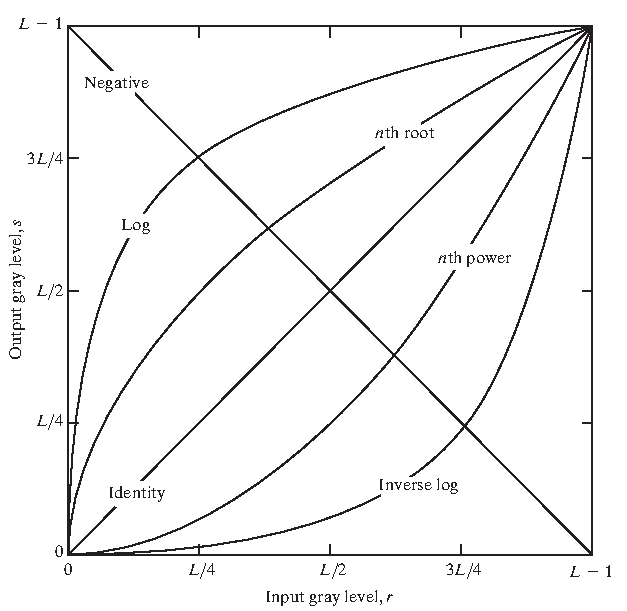
\includegraphics[width=.8\linewidth]{images/basic-transformations}
    \caption{Some basic grey-level transformations}
    \label{fig:basic-transformations}
\end{figure}

\subsubsection{Negative}
Inverts the intensity levels of the image (white becomes black and so on). Enhances details in dark regions.
\begin{equation}
    s = L - 1 - r
\end{equation}

\subsubsection{Log transformation}
Used to expand dark areas and compress bright areas, i.e. give more shadow detail. Good for displaying images with very large dynamic range.
\begin{equation}
    s = c \log(1 + r), \quad r \geq 0
\end{equation}

\subsubsection{Gamma transformation}
Can compress blacks or whites depending on the gamma value. Similar to the log transformation, but more versatile. Many devices have an inherent gamma transform response that can be compensated for by applying the opposite gamma transform. Can be used to improve detail by darkening a washed-out image or brightening a too dark image.
\begin{equation}
    s = c r^\gamma
\end{equation}

\subsubsection{Piecewise linear transformation}
Use a piecewise linear function as the transformation (as opposed to the smooth transformations in Figure \ref{fig:basic-transformations}). Many uses, depending on the function:
\begin{itemize}
    \item Contrast stretching: Increase the dynamic range of the grey levels, similar to a a sigmoid function. (Can also be done with a smooth function.)
    \item Grey-level slicing: Highlight a range of grey-levels. Either leave other values as they are or darken all other values.
    \item Bit-plane slicing: Consider e.g. an 8-bit image to be made of 8 bit `planes'. Extracting one or some of these is called bit-plane slicing. The most significant plane can be extracted to form a binary black or white image, for instance.
\end{itemize}

%%%%%%%%%%%%%%%%%%%%%%%%%%%%%%%%%%%%%%%%%%%%%%%%%%%%%%%%%%%%
\subsection{Histogram processing}

\subsubsection{Histogram equalization}
The cumulative probability density (CPD) of an image is
\begin{equation}
    F(r) = \int_0^r p_r (w) \dif w ,
\end{equation}
which leads to the transformation
\begin{equation}
    s = T(r) = (L-1) F(r).
\end{equation}
$p_r(w)$ is the probability for a pixel to be of intensity $w$. This transformation makes the histogram flat/uniform, which improves contrast by utilizing darks and lights equally much, rather than compressing the image into midtones.

\subsubsection{Histogram matching}
Sometimes you don't want a flat histogram, but a specific, nonflat distribution. Histogram matching is the method of transforming an image so that its histogram matches any given distribution.

\subsubsection{Local histogram processing}
The previous two methods are global, but sometimes a local method is better. This is done by iterating through pixels, looking at and changing the histogram of its neighborhood, and updating the pixel value according to the altered local histogram. An example is histogram equalization for a small moving window.

%!TEX root = TDT4265-Summary.tex
\section{Spatial filtering}

%%%%%%%%%%%%%%%%%%%%%%%%%%%%%%%%%%%%%%%%%%%%%%%%%%%%%%%%%%%%
\subsection{Fundamentals of spatial filtering}

\subsubsection{Mechanics of spatial filtering}
A spatial filter consists of a neighborhood and an operation performed on the pixels in the neighborhood. A \emph{linear filter} requires a linear operation, such as summation. Otherwise, it is a \emph{nonlinear filter}.

\subsubsection{Spatial correlation and convolution}
Neighborhood operations where each output pixel is a weighted sum of neighbors to the corresponding input pixel. The weights are stored in a matrix called filter, mask or kernel. Correlation and convolution are the same except for the fact that the filter is rotated $180 \degree$ for convolution.

If the input image is a discrete unit impulse (all zeros except a single `1' value), the output of convolution is the filter itself at the position of the unit impulse. Correlation has the same result, but the output is rotated 180 degrees. Convolution is commutative and associative:
\begin{gather}
    f \conv g = g \conv f \\
    f \conv (g \conv h) = (f \conv g) \conv h
\end{gather}
However, correlation is \emph{not}.

Because of the similarity of the operations, often only \eqref{eq:corr} is implemented, and the filter is rotated beforehand for convolution.

\paragraph{Correlation}
\begin{equation}\label{eq:corr}
    w(x,y) \corr f(x,y)
    =
    \sum_{s=-a}^{a}
    \sum_{t=-b}^{b}
    w(s,t) f(x+s, y+t)
\end{equation}

\paragraph{Convolution}
\begin{equation}\label{eq:conv}
    w(x,y) \conv f(x,y)
    =
    \sum_{s=-a}^{a}
    \sum_{t=-b}^{b}
    w(s,t) f(x-s, y-t)
\end{equation}

%%%%%%%%%%%%%%%%%%%%%%%%%%%%%%%%%%%%%%%%%%%%%%%%%%%%%%%%%%%%
\subsection{Smoothing spatial filters}
Used for blurring and noise reduction. Blurring can e.g. remove small, unwanted details before object detection.

Smoothing linear filters take an average of pixels under the mask. Also called averaging or lowpass filters. A typical filter is
\begin{equation}
    \frac{1}{9}
    \cdot
    \begin{BMAT}(e){|c|c|c|}{|c|c|c|}
        1 & 1 & 1 \\
        1 & 1 & 1 \\
        1 & 1 & 1
    \end{BMAT}
    \, .
\end{equation}
Such filters where all coefficients are equal are called box filters. Another possibility is a weighted average such as
\begin{equation}
    \frac{1}{16}
    \cdot
    \begin{BMAT}(e){|c|c|c|}{|c|c|c|}
        1 & 2 & 1 \\
        2 & 4 & 2 \\
        1 & 2 & 1
    \end{BMAT}
    \, ,
\end{equation}
which can smooth an image with less blurring than a box filter.

\subsubsection{Median filter}
A nonlinear filter, good for removing e.g. salt-and-pepper noise. Does not blur sharp edges. Method:
\begin{enumerate}
    \item Order pixels in the neighborhood by intensity.
    \item Replace center pixel with median intensity.
\end{enumerate}

%%%%%%%%%%%%%%%%%%%%%%%%%%%%%%%%%%%%%%%%%%%%%%%%%%%%%%%%%%%%
\subsection{Sharpening spatial filters}

Just like smoothing/averaging is analogous to integration, sharpening can be done by differentiation. Some requirements for a sharpening filter based on the first derivative are
\begin{itemize}
    \item zero in constant areas,
    \item nonzero at the onset and end of an intensity ramp, and
    \item nonzero during an intensity ramp.
\end{itemize}
Requirements for a secord-order derivative filter are the same, with the difference that it must be zero during ramps. The one-dimensional definitions
\begin{equation}
\begin{split}
    \pd{f}{x}    &= f(x+1) - f(x) \\
    \pd[2]{f}{x} &= f(x+1) + f(x-1) - 2f(x)
\end{split}
\end{equation}
satisfy these requirements.

\subsubsection{Image sharpening with the Laplacian}
For 2D images, sharpening filters can be based on the Laplacian
\begin{equation}
    \nabla^2 f = \pd[2]{f}{x} + \pd[2]{f}{y} .
\end{equation}

Some common filters are:
\begin{equation}\label{eq:laplacian-filters}
    \begin{BMAT}(e){|c|c|c|}{|c|c|c|}
        0 &  1 & 0 \\
        1 & -4 & 1 \\
        0 &  1 & 0
    \end{BMAT}
    \quad
    \begin{BMAT}(e){|c|c|c|}{|c|c|c|}
        1 &  1 & 1 \\
        1 & -8 & 1 \\
        1 &  1 & 1
    \end{BMAT}
    \quad
    \begin{BMAT}(e){|c|c|c|}{|c|c|c|}
         0 & -1 &  0 \\
        -1 &  4 & -1 \\
         0 & -1 &  0
    \end{BMAT}
    \quad
    \begin{BMAT}(e){|c|c|c|}{|c|c|c|}
        -1 & -1 & -1 \\
        -1 &  8 & -1 \\
        -1 & -1 & -1
    \end{BMAT}
\end{equation}

The sharpened image is obtained by taking the sum of the original and the filtered image:
\begin{equation}
    g(x,y) = f(x,y) + c [\nabla^2 f(x,y)]
\end{equation}
where $c$ is $-1$ if the center element of the filter is negative, and $1$ otherwise.

\subsubsection{Unsharp masking and highboost filtering}\label{sssec:unsharp-highboost-spatial}
Unsharp masking sort of goes in the opposite direction of Laplacian sharpening: First blur the image, and subtract the blurred from the original to get a an unsharp mask $g\sub{mask}(x,y) = f(x,y) - \overline{f}(x,y)$. Finally add the mask to the original:
\begin{equation}\label{eq:unsharp-masking}
    g(x,y) = f(x,y) + k \cdot g\sub{mask}(x,y)
\end{equation}
Unsharp masking is strictly speaking only for $k = 1$. With $k > 1$, we have highboost filtering, and you can also lessen the effect with $k < 1$. The result is a sharpened image, because you remove unsharpness, which increases corner contrast.

\subsubsection{Image sharpening with the Gradient}
Section \ref{sssec:edge-detection} defines the gradient. Its magnitude
\begin{equation}
    M(x,y) = \sqrt{g_x^2 + g_y^2} \approx \abs{g_x} + \abs{g_y}
\end{equation}
forms a gradient magnitude image. An example of masks that approximate this is the Sobel operator \eqref{eq:sobel}.

%%%%%%%%%%%%%%%%%%%%%%%%%%%%%%%%%%%%%%%%%%%%%%%%%%%%%%%%%%%%
\subsection[Combining methods]{Combining spatial enhancement methods}
In the real world, you need to use several methods to solve a task. One example is to first sharpen the image, then enhance the dynamic range.

%!TEX root = TDT4265-Summary.tex
\section{Frequency filtering}

\begin{equation}
    \euler^{\ramuno \theta}
    =
    \cos \theta
    +
    \ramuno \sin \theta
\end{equation}

%%%%%%%%%%%%%%%%%%%%%%%%%%%%%%%%%%%%%%%%%%%%%%%%%%%%%%%%%%%%
\subsection{Fourier transformation}

\subsubsection{1D continuous Fourier transform (CFT)}
The following equations define the forward and backward CFTs:
\begin{gather}
    F(u) = \int_{-\infty}^{\infty} f(x) \euler^{-2 \pi u x} \dif x \\
    f(x) = \int_{-\infty}^{\infty} F(u) \euler^{\ramuno 2 \pi u x} \dif u \\
\end{gather}
In many fields $f(x)$ is a function of time, but in image processing it is usually a function that maps from spatial position in an image to image intensity. Then $F(u)$ is a complex function of frequency, with a magnitude and phase (usually only magnitude is displayed).

\subsubsection{2D discrete Fourier transform (DFT)}
Digital images have discrete values, and are 2D, so we need a 2D DFT to convert them to the frequency domain. For an image of size $M \times N$, it is
\begin{equation}
    F(u,v)
    =
    \sum_{x=0}^{M-1}
    \sum_{y=0}^{N-1}
    f(x,y)
    \euler^{-\ramuno 2 \pi (\frac{ux}{N}+\frac{vy}{N})}
\end{equation}
and the inverse transform is
\begin{equation}
    f(x,y)
    =
    \frac{1}{MN}
    \sum_{u=0}^{M-1}
    \sum_{v=0}^{N-1}
    F(u,v)
    \euler^{\ramuno 2 \pi (\frac{ux}{M}+\frac{vy}{N})}
    .
\end{equation}

\begin{figure}[htbp]
    \hfill
    \subfigure[Intensity image]{
\includegraphics[width=.45\linewidth]{images/sin3.png}}
    \hfill
    \subfigure[Frequency image]{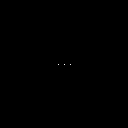
\includegraphics[width=.45\linewidth]{images/sin3real.png}}
    \hfill
    \caption{An image and its Fourier transform}
\end{figure}

%%%%%%%%%%%%%%%%%%%%%%%%%%%%%%%%%%%%%%%%%%%%%%%%%%%%%%%%%%%%
\subsection{Convolution}

\paragraph{Convolution theorem} Convolution in one domain is equal to multiplication in the other:
\begin{equation}\label{eq:convolution-theorem}
\begin{split}
    h(x) \conv f(x) &\iff H(x) \cdot F(x) \\
    h(x) \cdot f(x) &\iff H(x) \conv F(x)
\end{split}
\end{equation}

%%%%%%%%%%%%%%%%%%%%%%%%%%%%%%%%%%%%%%%%%%%%%%%%%%%%%%%%%%%%
\subsection{The sampling theorem}
If samples are taken at a rate over twice the highest frequency of a function, it can be recreated without loss of information. This limit is the sampling theorem:
\begin{equation}
    \frac{1}{\Delta T} > 2 \mu\sub{max}
\end{equation}

%%%%%%%%%%%%%%%%%%%%%%%%%%%%%%%%%%%%%%%%%%%%%%%%%%%%%%%%%%%%
\subsection{Basics of frequency domain filtering}
Filtering of an image $F(u,v)$ in the frequency domain with a filter $H(u,v)$ is done by
\begin{equation}
    g(x,y) = \fourier^{-1}[H(u,v) F(u,v)]
\end{equation}
where $H$ is a matrix of equal size to the image. (The multiplication $H F$ is done elementwise.)

\paragraph{Shifting}
To obtain a centered Fourier transform, multiply the image by $(-1)^{x+y}$ before transforming. Then $F(0,0)$ will be at the center. Alternatively swap the quadrants after transforming.

%%%%%%%%%%%%%%%%%%%%%%%%%%%%%%%%%%%%%%%%%%%%%%%%%%%%%%%%%%%%
\subsection{Frequency domain smoothing}

\subsubsection{Ideal low-pass filter (ILPF)}
An ILPF is a filter with no attenuation for frequencies below a threshold (the \emph{cutoff frequency}), and full attenuation for all frequencies above:
\begin{equation}
    H(u,v) =
    \begin{cases}
        1 \quad\mbox{if } D(u,v) \leq D_0 \\
        0 \quad\mbox{if } D(u,v) >    D_0
    \end{cases}
\end{equation}
The spatial representation of the ILPF is the $\sinc$ function (in 2D, that means any cross-section through the origin is a $\sinc$ function).

The convolution theorem \eqref{eq:convolution-theorem} then reveals why the ringing effect occurs: Multiplying with an ILPF in the frequency domain is equivalent to convolving with a $\sinc$ filter (Figure \ref{fig:sinc}) in the spatial domain.

\begin{figure}[htbp]
    \centering
    % 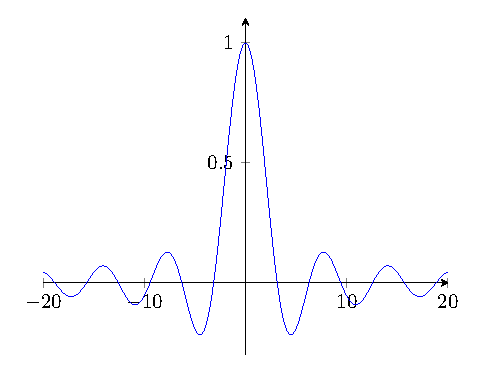
\includegraphics[width=.8\linewidth]{images/sinc_x_plot}
    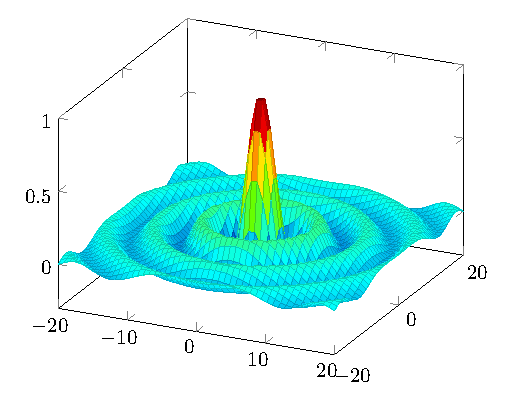
\includegraphics[width=.8\linewidth]{images/sinc_2d_plot}
    \caption{The $\sinc$ function}
    \label{fig:sinc}
\end{figure}

\subsubsection{Butterworth low-pass filter (BLPF)}
Defined as
\begin{equation}
    H(u,v)
    =
    \frac{1}{1 + [D(u,v)/D_0]^{2n}}
\end{equation}
where $n$ is the order and $D(u,v)$ is the distance in the frequency domain between $(u,v)$ and the center. This gives a smooth cutoff, which reduces ringing (depending on order). Order 1 has no ringing, 2 very little, and higher orders may have visible ringing. (A BLPF with $n = \infty$ is equal to an ILPF.)

\subsubsection{Gaussian low-pass filter (GLPF)}
Given in 2D as
\begin{equation}
    H(u,v) = \euler^{-\frac{D^2(u,v)}{2 D_0}}.
\end{equation}

The inverse Fourier of this is also a Gaussian function, so it will have no ringing. It's pretty nice.

\subsubsection{Some examples of lowpass filtering}
\begin{itemize}
    \item Smoothing digitized text to fill gaps and improve legibility, especially for machine processing.
    \item Cosmetic processing, such as softening skin on images of people.
    \item Removing artifacts, such as noise and scan lines.
    \item However, smoothing is mostly used for preprocessing.
\end{itemize}

%%%%%%%%%%%%%%%%%%%%%%%%%%%%%%%%%%%%%%%%%%%%%%%%%%%%%%%%%%%%
\subsection{Frequency domain sharpening}
Done with high-pass filters, which are pretty much the opposite of low-pass filters:
\begin{equation}\label{eq:frequency-hp-lp-relation}
    H\sub{highpass}(u,v) = 1 - H\sub{lowpass}(u,v)
\end{equation}

\subsubsection{Ideal high-pass filter (IHPF)}
Defined as
\begin{equation}
    H(u,v) =
    \begin{cases}
        0 \quad\mbox{if } D(u,v) \leq D_0 \\
        1 \quad\mbox{if } D(u,v) >    D_0
    \end{cases}
\end{equation}

\subsubsection{Butterworth high-pass filter (BHPF)}
\begin{equation}
    H(u,v) =
    \frac{1}{1 + [D_0 / D(u,v)]^{2n}}
\end{equation}

\subsubsection{Gaussian high-pass filter (GHPF)}
\begin{equation}
    H(u,v) = 1 - \euler^{-\frac{D^2(u,v)}{2 D_0^2}}
\end{equation}

\subsubsection{Frequency domain Laplacian filter}
The Laplacian works the same way in the frequency domain as in the spatial domain. With
\begin{equation}
    H(u,v) = -4\pi^2(u^2 + v^2)
\end{equation}
the Laplacian image is
\begin{equation}
    \nabla^2 f(x,y) = \fourier^{-1} \left\{ H(u,v) F(u,v) \right\}
\end{equation}
and the enhanced image is
\begin{equation}
    g(x,y) = f(x,y) + c \nabla^2 f(x,y)
\end{equation}

\subsubsection{Unsharp masking, highboost filtering, high-frequency emphasis filtering}
Like in the spatial domain \eqref{eq:unsharp-masking}, unsharp masking and highboost filtering can be be done in the frequency domain:
\begin{equation}
\begin{split}
    g(x,y)
    &=
    \fourier^{-1}
    \left\{
        \left[
            1 + k \cdot [1 - H\sub{LP}(u,v)]
        \right]
        F(u,v)
    \right\} \\
    &=
    \fourier^{-1}
    \left\{
        [1 + k \cdot H\sub{HP}(u,v)] F(u,v)
    \right\}
\end{split}
\end{equation}
Remember \eqref{eq:frequency-hp-lp-relation}. This leads to the high-frequency emphasis filter
\begin{equation}
    g(x,y)
    =
    \fourier^{-1}
    \left\{
        [k_1 + k_2 \cdot H\sub{HP}(u,v)] F(u,v)
    \right\}
\end{equation}
where $k_1 \geq 0$ is the DC term, and $k_2 \geq 0$ sets the contribution of high frequencies. By setting a nonzero DC term, the low frequency grey levels is not lost. High-frequency emphasis filtering followed by histogram equalization can enhance clarity and detail significantly, and is useful for e.g. X-ray images.

%%%%%%%%%%%%%%%%%%%%%%%%%%%%%%%%%%%%%%%%%%%%%%%%%%%%%%%%%%%%
\subsection{Selective filters}
These filters only affect parts of the frequency spectrum.

\subsubsection{Bandreject and bandpass}
Filters that remove all frequencies inside or outside a given range. Like normal filters, these can be created as ideal, Butterworth, or Gaussian filters.

\subsubsection{Notch filters}
These filters reject (or pass) frequencies at chosen locations in the frequency rectangle. A common example is removing periodic noise, such as moiré.

%!TEX root = TDT4265-Summary.tex
\section{Morphological image processing}
Morphology is image manipulation via set theory. It's pretty cool. Sort of like spatial filtering, but with nonlinear operations.

%%%%%%%%%%%%%%%%%%%%%%%%%%%%%%%%%%%%%%%%%%%%%%%%%%%%%%%%%%%%
\subsection{Preliminaries}
In morphology, images are represented as sets. Usually images are binary, and the set of an image is the set of 1-valued pixels, defined on $\mathbb{Z}^2$. An extension in $\mathbb{Z}^3$ to greyscale exists, and also to color and so on.

\subsubsection{Some set theory}
\begin{itemize}
    \item The absolute complement of a set $A$ is
    \begin{equation}
        A^c = \{ w | w \notin A \},
    \end{equation}
    which is all elements outside of $A$.
    \item The relative complement between two sets $A$ and $B$ is
    \begin{equation}
        A \setminus B = \{ w | w \in A, w \notin B \},
    \end{equation}
    which is all elements that are \emph{only} in $A$.
    \item The reflection (180 degree rotation) of a set is
    \begin{equation}
        \hat{B} = \{ w | w = -b \mbox{ for } b \in B \}.
    \end{equation}
    \item The translation of a set $A$ by a vector $z = (z_1, z_2)$ is
    \begin{equation}
        (B)_z = \{ c | c = b + z \mbox{ for } b \in B \}
    \end{equation}
\end{itemize}

\subsubsection{Structuring elements (SEs)}
An SE is a small subimage or subset that is used to find properties of the image. They are usually symmetric and with their center defined in the middle.

%%%%%%%%%%%%%%%%%%%%%%%%%%%%%%%%%%%%%%%%%%%%%%%%%%%%%%%%%%%%
\subsection{Erosion and dilation}

\subsubsection{Erosion}
The erosion of $A$ by $B$ is defined as
\begin{equation}
    A \erode B = \left\{ z | (B)_z \subseteq A \right\},
\end{equation}
which is the set of all points where $B$ is completely inside $A$. ($A$ is an image and $B$ is an SE.) The operation shrinks objects, and removes anything smaller/thinner than the SE, such as thin lines.

\subsubsection{Dilation}
The dilation of $A$ by $B$ is defined as
\begin{equation}
    A \dilate B = \left\{ z | (\hat{B})_z \cap A \neq \emptyset \right\}
\end{equation}
which is the set of all points where $\hat{B}$ (the reflection of $B$) overlaps with $A$ by at least one element. This operation grows objects, and can fill gaps and small holes.

\subsubsection{Duality}
Erosion and dilation are dual operations:
\begin{equation}
\begin{split}
    (A \erode  B)^c &= A^c \dilate \hat{B} \\
    (A \dilate B)^c &= A^c \erode  \hat{B} \\
\end{split}
\end{equation}
This is useful for symmetric SEs ($\hat{B} = B$), because then we can erode $A$ by instead dilating the background $A^c$.

%%%%%%%%%%%%%%%%%%%%%%%%%%%%%%%%%%%%%%%%%%%%%%%%%%%%%%%%%%%%
\subsection{Opening and closing}\label{ssec:open-close}
\emph{Opening} is defined as
\begin{subequations}
\begin{align}
    A \open B &= (A \erode B) \dilate B \\
              &= \bigcup \left\{ (B)_z | (B)_z \subseteq A \right\} \label{eq:opening-as-set}
\end{align}
\end{subequations}
It is analogous to the area defined by moving a ball (or other shape) along the inner boundary of a set, as in Figure \ref{fig:openclose}. Equation \eqref{eq:opening-as-set} shows that opening can be expressed as ``all translates of $B$ that fit inside $A$''. Used for e.g. removing thin connections between components and removing noise pixels.

\emph{Closing} is defined as
\begin{equation}
    A \close B = (A \dilate B) \erode B,
\end{equation}
which is analogous to the area defined by moving e.g. a ball along the outer boundary of a set, as in Figure \ref{fig:openclose}. Used for e.g. filling holes.

\begin{figure}[htbp]
    \centering
    \subfigure[Opening]{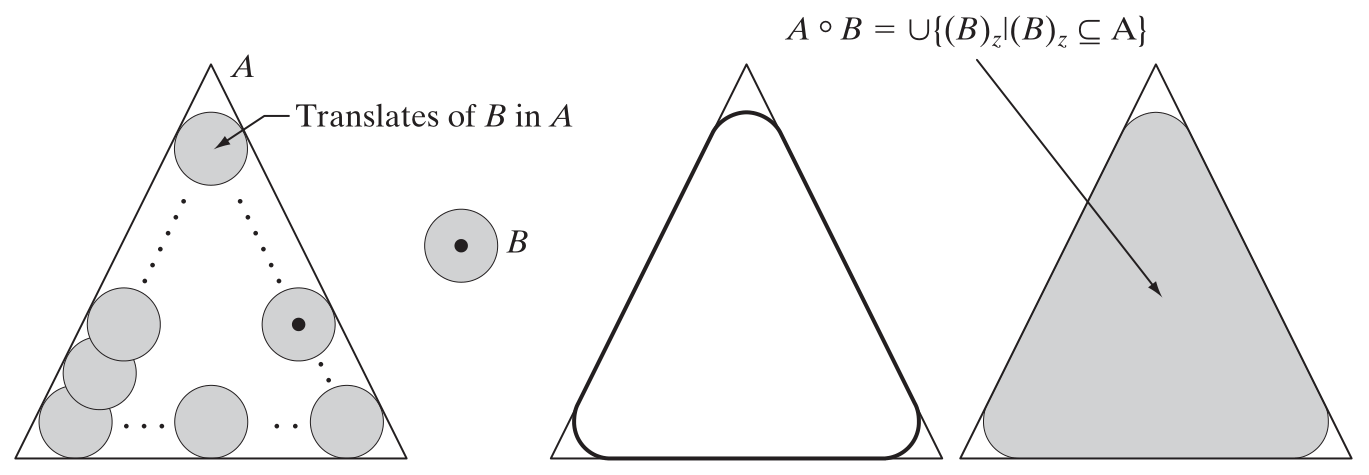
\includegraphics[width=.9\linewidth]{images/opening.png}} \\
    \subfigure[Closing]{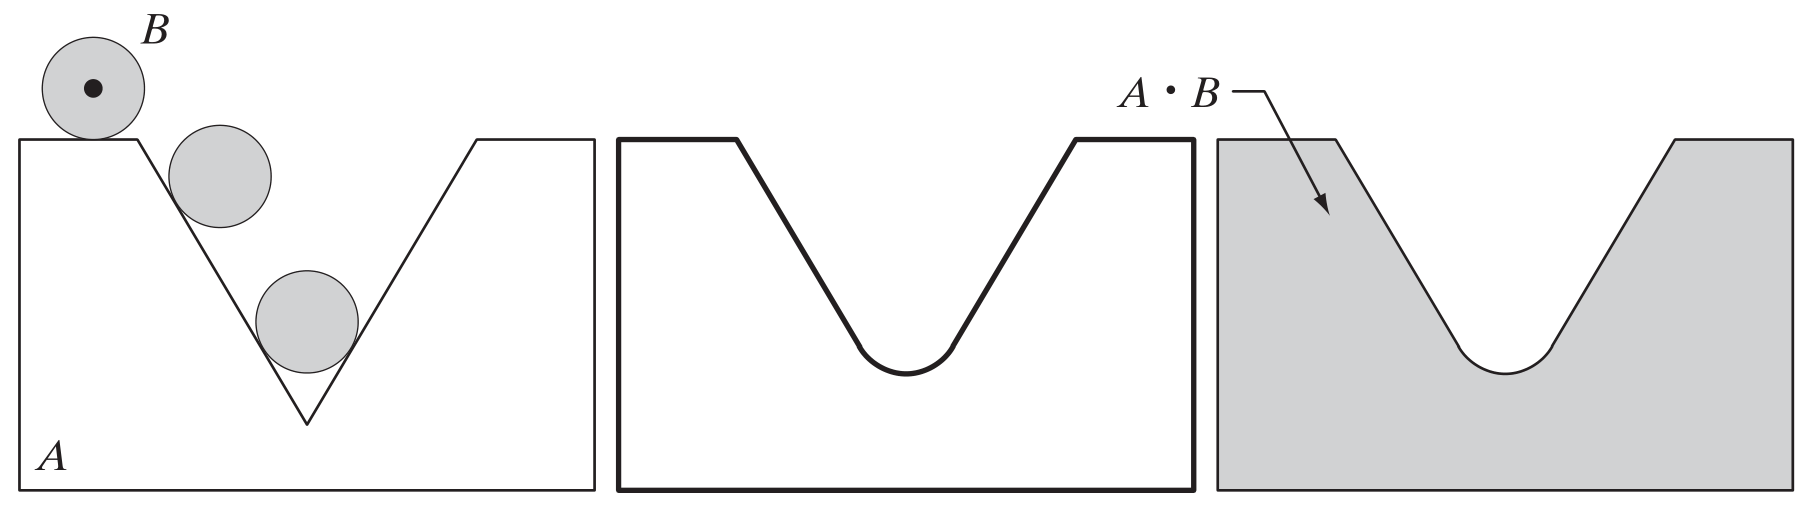
\includegraphics[width=.9\linewidth]{images/closing.png}}
    \caption{Analogies to the opening and closing operations}
    \label{fig:openclose}
\end{figure}

Note that both opening and closing are idempotent operations.

\paragraph{Combining opening and closing}
Opening followed by closing can remove noise, both specks of object pixels on the background and background pixels where there should be object. However, some connectivity may be lost.

%%%%%%%%%%%%%%%%%%%%%%%%%%%%%%%%%%%%%%%%%%%%%%%%%%%%%%%%%%%%
\subsection{The hit-or-miss transformation}
A basic tool for shape detection. Let $B = (B_1, B_2)$, $B_1$ be an object, and $B_2$ its background. Then the matches of $B$ in $A$ is
\begin{equation}
    A \match B = (A \erode B_1) \cap (A^c \erode B_2).
\end{equation}
The set $(A \erode B_1)$ are all locations where the object fits in, and $(A^c \erode B_2)$ are all locations where the background fits. Locations where both fit are locations of all shapes in $A$ that perfectly match $B$. We assume that each object we want to find is separate from the other objects, and therefore each has a complete local background at least one pixel wide.

%%%%%%%%%%%%%%%%%%%%%%%%%%%%%%%%%%%%%%%%%%%%%%%%%%%%%%%%%%%%
\subsection{Some basic morphological algorithms}
Now we can finally use this stuff.

\subsubsection{Boundary extraction}
Get the boundary by subracting the eroded image from the original.
\begin{equation}
    \beta(A) = A - (A \erode B)
\end{equation}
The erosion gives a ``smaller'' version of $A$, and subtracting that from the image leaves only the border.

\subsubsection{Hole filling}
Same principle as in Section \ref{sec:extract-connected} below.
\begin{equation}
    X_k = (X_{k-1} \dilate B) \cap A^c
\end{equation}
The seed pixel must be in a hole. It will grow until it fills the hole. Stop when no further change happens.

\subsubsection{Extraction of connected components}\label{sec:extract-connected}
Done by iteration:
\begin{equation}
    X_k = (X_{k-1} \dilate B) \cap A
\end{equation}
Choose a starting pixel (seed) $X_0$. Dilate $X_0$, but only keep the pixels that are in the original. Continue dilating and only keeping pixels present in $A$ until convergence.

\subsubsection{Convex hull}\label{sec:convex-hull}
A set is convex if any line segment between two points in the set lies fully within the set. The \emph{convex hull} $H$ of a set $S$ is the smallest convex set containing $S$. The difference $H - S$ is the \emph{convex decifiency} of $S$. It can be computed by iterating
\begin{equation}
    X_k^i = (X_{k-1} \match B^i) \cup A
    ,\quad i = 1,2,3,4
    ,\quad k = 1,2,\dots
\end{equation}
with $X_0^i = A$ and $B^i$ being as shown in Figure \ref{fig:convex-hull-SE}. For each SE, let $D^i = X_k^i$ when its iteration converges. Then the convex hull is
\begin{equation}
    C(A) = \bigcup_{i=4}^{4} D^i
\end{equation}

\begin{figure}[htbp]
    \centering
    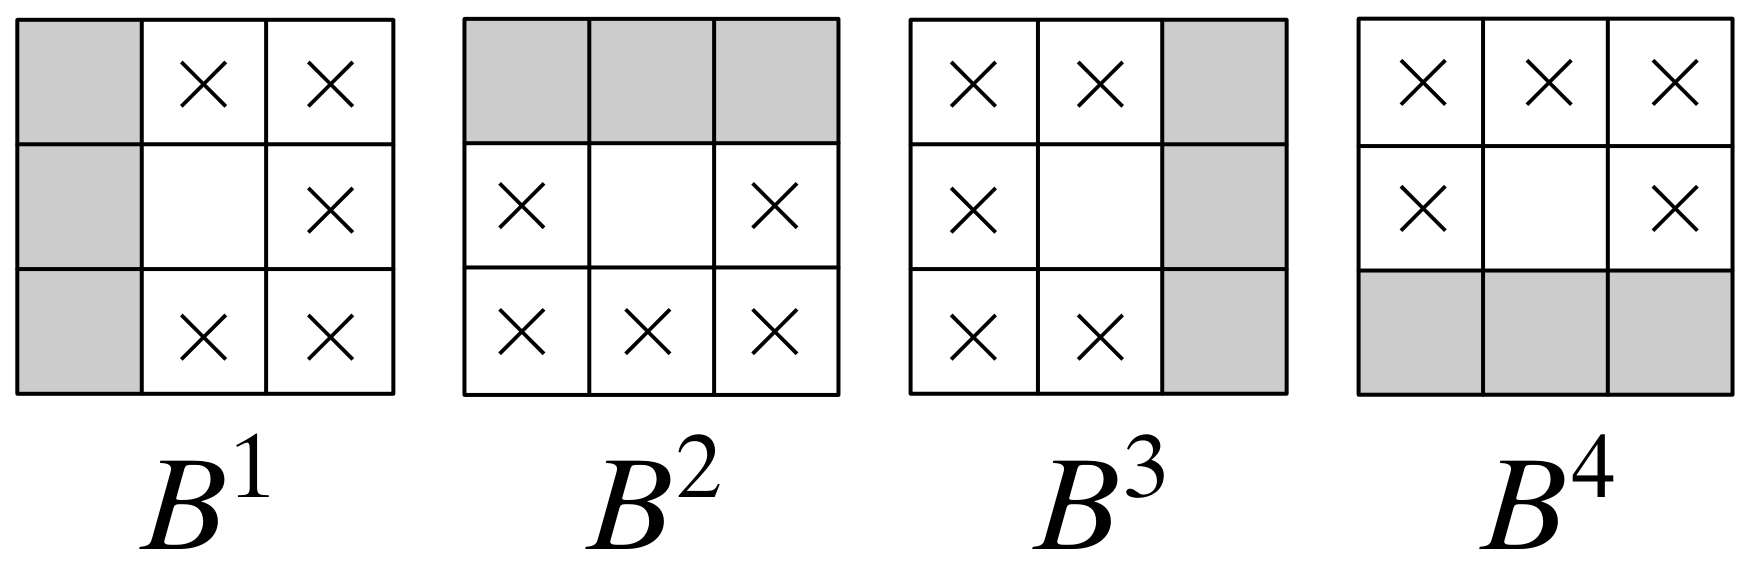
\includegraphics[width=.5\linewidth]{images/SE-for-convex-hull.png}
    \caption{SEs for convex hull extraction}
    \label{fig:convex-hull-SE}
\end{figure}

\subsubsection{Thinning}\label{sec:thinning}
Used e.g. for skeletonization and to thin edge detector output. It is defined in terms of the hit-or-miss transformation as
\begin{equation}
    A \thin B = A \cap (A \match B)^c
\end{equation}
with a sequence of SEs
\begin{equation}
    \{ B \} = \{ B^1, \dots, B^n \}
\end{equation}
where $B^i$ is a rotated $B^{i-1}$. Then just keep applying hit-or-miss with $B$ repeatedly, until continuing has no effect.

One pass of thinning is written as
\begin{equation}
    A \thin \{ B \} = ((\dots ((A \thin B^1) \thin B^2) \dots ) \thin B^n)
\end{equation}

\subsubsection{Thickening}
Thickening is the dual of thinning:
\begin{equation}
    A \thick B = A \cup (A \match B)
\end{equation}

\subsubsection{Skeletons}
The skeleton is
\begin{equation}
    S(A) = \bigcup_{k=0}^{K} (A \erode kB) - (A \erode kB) \open B
\end{equation}
where $B$ is an SE and $(A \erode kB)$ indicates $k$ successive erosions of $A$. $K$ is the number of erosions possible before resulting in the empty set.

\subsubsection{Pruning}
Skeletons often have unwanted ``spurs''. Assuming the spurs are sufficiently small, pruning can remove them. We perform thinning with SEs designed to only detect end points.
\begin{equation}
    X_1 = A \thin \{B\}
\end{equation}
The SEs used are shown in Figure \ref{fig:se-for-pruning}.

\begin{figure}[htbp]
    \centering
    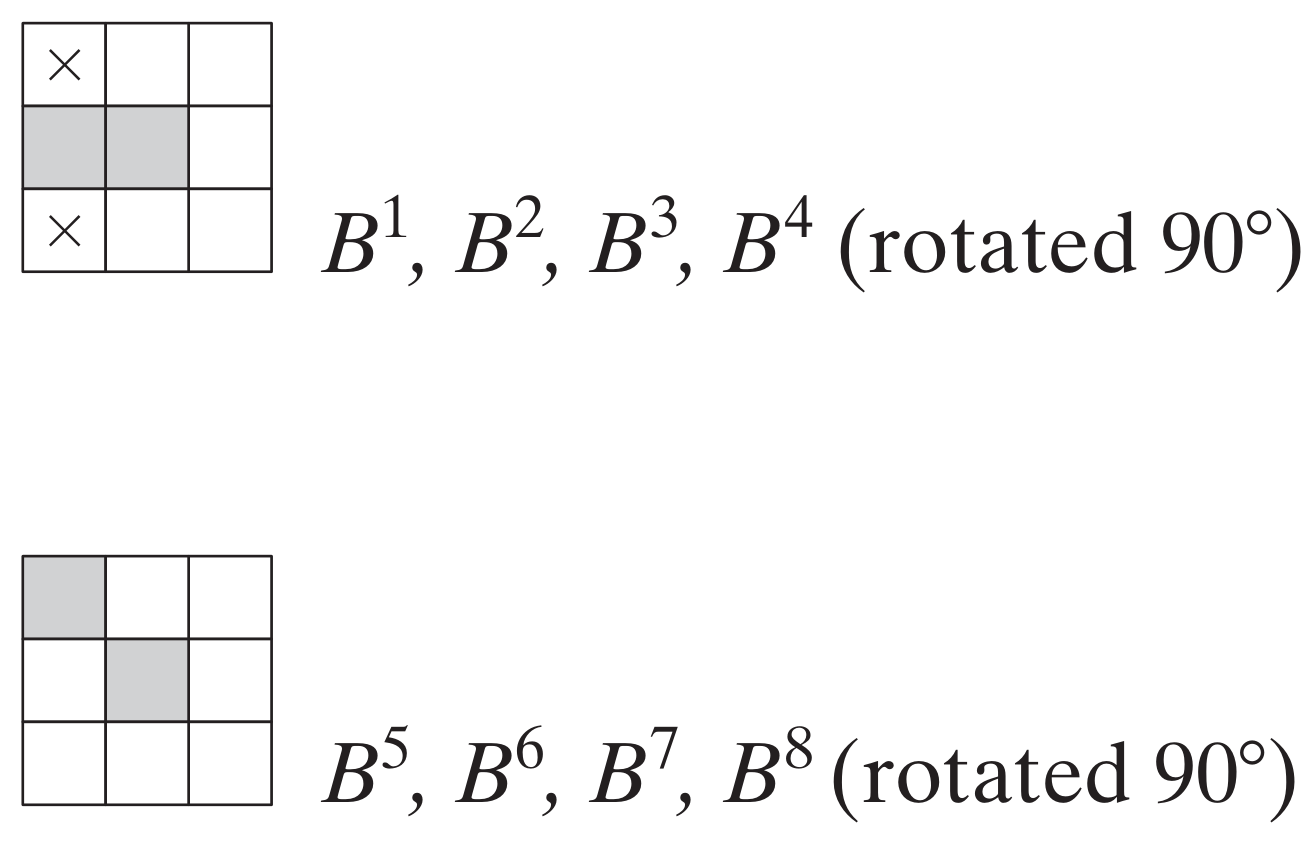
\includegraphics[width=0.5\linewidth]{images/SE-for-pruning.PNG}
    \caption{SEs for pruning}
    \label{fig:se-for-pruning}
\end{figure}

\subsubsection{Morphological reconstruction}
Uses two images, a marker $F$ with starting points, and a mask $G$ that constrains the transformation.

\paragraph{Geodesic dilation}
Geodesic dilation is the intersection of the mask and the dilated marker. One pass is
\begin{equation}\label{eq:geo-dilation}
    D_G^{(1)}(F) = (F \dilate B) \cap G.
\end{equation}
Several passes, denoted $D_G^{(n)}$, is just repeating the operation $n$ times.

\paragraph{Geodesic erosion}
Geodesic erosion is the union of the mask and the eroded marker. One pass is
\begin{equation}\label{eq:geo-erosion}
    E_G^{(1)}(F) = (F \erode B) \cup G.
\end{equation}

\paragraph{Morphological reconstruction by dilation}
Reconstruction by dilation is just repeating \eqref{eq:geo-dilation} until more passes have to effect:
\begin{equation}
    R_G^D(F) = D_G^{(k)}(F)
\end{equation}

\paragraph{Morphological reconstruction by erosion}
Same as by dilation, but using erosion:
\begin{equation}
    R_G^E(F) = E_G^{(k)}(F)
\end{equation}

\paragraph{Opening by reconstruction}
With normal opening (Section \ref{ssec:open-close}), erosion removes small things and dilation restores the original size/shape. Opening by reconstruction restores the precise original shape, and is done as reconstruction by dilation of $F$, from the erosion of size $n$ of $F$:
\begin{equation}
    O_R^{(n)}(F) = R_F^D \left[ (F \erode nB) \right]
\end{equation}
where $(F \erode nb)$ indicates $n$ erosions.

The SE for erosion $B$ determines the shapes we want to identify. The erosion itself leaves us with markers for all matching objects (because they are not removed by the erosion). Then, the image $F$ is used as a mask, and reconstruction is done by dilating the markers, subject to the mask. That way, all objects marked will be completely filled, and the result is removing all unmarked objects.

\paragraph{Filling holes}
With morphological reconstruction we can fill holes automatically, without knowing where they are. Create a marker image $F$ of zeros, except for the border, where it is $1 - I$. Then
\begin{equation}
    H = \left[ R_{I^c}^D(F) \right]^c
\end{equation}
is $I$ with all holes filled.

\paragraph{Border clearing}
Morphological reconstruction can also be used to remove objects connected to the borders of an image. Create a marker image $F$ that is equal to the input image $I$ at the border, and 0 elsewhere. We can extract all border-touching objects by the morphological reconstruction $R_I^D(F)$, and subtract it from the original to get an image without border objects $X$:
\begin{equation}
    X = I - R_I^D(F)
\end{equation}

\subsubsection{Summary}
We have now defined the following morphological operations:
\begin{itemize}
    \item Basic set operations:
    \begin{itemize}
        \item Translation
        \item Reflection
        \item Complement
        \item Difference
    \end{itemize}
    \item Basic morphological operations:
    \begin{itemize}
        \item Erosion
        \item Dilation
        \item Opening
        \item Closing
    \end{itemize}
    \item Complex morphological operations:
    \begin{itemize}
        \item Hit-or-miss transform
        \item Boundary extraction
        \item Hole filling
        \item Connected components
        \item Convex hull
        \item Thinning
        \item Thickening
        \item Skeletons
        \item Pruning
    \end{itemize}
    \item Morphological reconstruction operations:
    \begin{itemize}
        \item Geodesic dilation
        \item Geodesic erosion
        \item Morphological reconstruction by dilation
        \item Morphological reconstruction by erosion
        \item Opening by reconstruction
        \item Closing by reconstruction
        \item Hole filling
        \item Border clearing
    \end{itemize}
\end{itemize}

%%%%%%%%%%%%%%%%%%%%%%%%%%%%%%%%%%%%%%%%%%%%%%%%%%%%%%%%%%%%
\subsection{Grey-scale morphology}
We can dilate, erode, open, and close grey-scale images too! Now we use images $f(x,y)$ and SEs $b(x,y)$. The SEs can now be either flat (uniform) or nonflat. We stick to flat SEs for simplicity.

\subsubsection{Erosion and dilation}
Erosion of $f$ by a flat SE $b$ is the minimum value of the image in the region covered by the SE:
\begin{equation}
    \left[ f \erode b \right](x,y) = \min_{(s,t) \in b} \left\{ f(x+s, y+t) \right\}.
\end{equation}
Dilation is similarly
\begin{equation}
    \left[ f \dilate b \right](x,y) = \max_{(s,t) \in b}  \left\{ f(x-s, y-t) \right\},
\end{equation}
which uses  $\hat{b} = b(-x,-y)$.

\subsubsection{Opening and closing}\label{sssec:greyscale-open-close}
This is mathematically just as before:
\begin{subequations}
\begin{align}
    f \open b = (f \erode b) \dilate b \\
    f \close b = (f \dilate b) \erode b
\end{align}
\end{subequations}

Looking at the image as a topographic surface, opening is pushing the SE up from below, clipping all peaks where it doesn't fit, and closing is pushing the SE down from above, clipping all valleys where it doesn't fit. See Figure \ref{fig:greyscale-opening-closing}. This means that opening removes small, bright details, and closing removes small, dark details.

\begin{figure}[htbp]
    \centering
    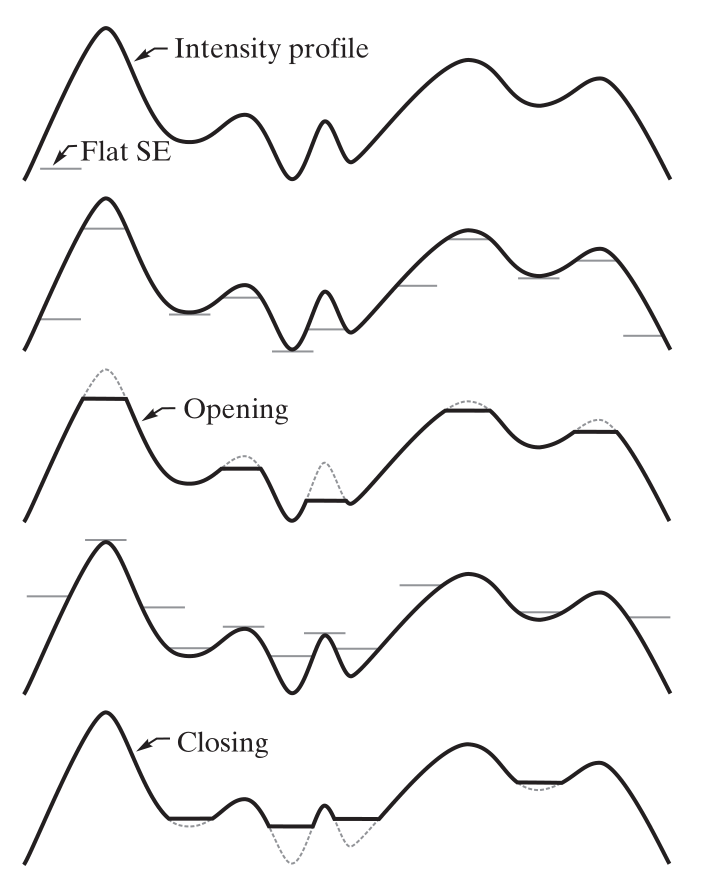
\includegraphics[width=0.8\linewidth]{images/greyscale-opening-closing}
    \caption{Analogy to opening and closing greyscale images}
    \label{fig:greyscale-opening-closing}
\end{figure}

\subsubsection{Some basic greyscale morphological algorithms}

\paragraph{Smoothing}
The ``small bright/dark details'' mentioned in Section \ref{sssec:greyscale-open-close} might be noise. This means we can remove this type of noise by opening and then closing. The size of the SE then sets a threshold for what is image and what is noise.

\paragraph{Morphological gradient}
The morphological gradient is
\begin{equation}
    g = (f \dilate b) - (f \erode b).
\end{equation}
The dilation thickens objects in the image, and the erosion shrinks them. Differencing these emphasises edges and removes homogenous areas, which gives a gradientlike effect.

\paragraph{Top-hat and bottom-hat transformations}\label{par:top-hat}
Subtracting the opening of an image from the image itself defined the top-hat transformation
\begin{equation}
    T\sub{hat}(f) = f - (f \open b).
\end{equation}
The bottom-hat transformation is defined similarly:
\begin{equation}
    B\sub{hat}(f) = (f \close b) - f
\end{equation}

Top-hat can isolate light objects on a dark background, and bottom-hat does the opposite. This is a type of segmentation, and works well even with uneven lightning.

Opening with an SE that is too large to fit in the objects you want to segment will remove all such objects and leave only an approximation of the background, including any uneven lightning. If you subtract the approximate background from the original, the unevenness will be reduced, and now thresholding methods can be used with success.

\paragraph{Granulometry}
(Assuming light objects on a dark background.) Open the image with gradually larger SEs, and compute the sum of pixel values. As the SEs grow larger than the objects, they disappear, and the pixel sum decreases. Plotting pixel sum against SE size indicates by peaks in the plot the predominant sizes of objects in the image. This can be used to simply get the size distribution of objects, but also to identify defect objects (sizewise).

\paragraph{Textural segmentation}
(Assuming light objects on a dark background.) Textural segmentation is to divide an image into regions based on their texture contents. If you have an image with some coarse and some fine texture, you can close it with an SE large enough to remove the fine objects. Then open it with an SE large enough to fill the gaps between the coarse objects. Now coarse areas are dark, and fine areas are bright, and the boundary can be extracted by e.g. a morph. gradient.

\subsubsection{Greyscale morphological reconstruction}
Let $f$ be the marker, and $g$ be the mask. The basic operations are similar to their black-and-white counterparts.
\begin{itemize}
    \item Geodesic dilation:
    \begin{equation}
        D_g^{(1)}(f) = (f \dilate b) \wedge g
    \end{equation}
    \item Geodesic erosion:
    \begin{equation}
        E_g^{(1)}(f) = (f \erode b) \vee g
    \end{equation}
    \item Reconstruction by dilation:
    \begin{equation}
        R_g^D(f) = D_g^{(k)}(f)
    \end{equation}
    \item Reconstruction by erosion:
    \begin{equation}
        R_g^E(f) = E_g^{(k)}(f)
    \end{equation}
    \item Opening by reconstruction:
    \begin{equation}
        O_R^{(n)}(f) = R_f^D \left[ (f \erode nb) \right]
    \end{equation}
    \item Closing by reconstruction:
    \begin{equation}
        C_R^{(n)}(f) = R_f^E \left[ (f \dilate nb) \right]
    \end{equation}
\end{itemize}

\paragraph{Top-hat by reconstruction}
This method consists of subtracting an image's opening by reconstruction from the image.

%!TEX root = TDT4265-Summary.tex
\section{Image segmentation}\label{sec:segmentation}
Segmentation divides an image into the regions or objects it consists of. Most algorithms here are based on intensity discontinuity and similarity.

%%%%%%%%%%%%%%%%%%%%%%%%%%%%%%%%%%%%%%%%%%%%%%%%%%%%%%%%%%%%
\subsection{Fundamentals}\label{ssec:segmentation-fundamentals}
We pretty much just divide an image $R$ into $n$ regions $R_1 \dots R_n$, and require the following to hold:
\begin{itemize}
    \item The union of all regions is equal to the whole image.
    \item Each region is a connected set.
    \item Each region is disjoint from the others.
    \item Some predicate\footnote{A predicate can be e.g. the that the intensity of each pixel is in a certain range.} is true for each region separately.
    \item The predicate is false for the union of any adjacent regions.
\end{itemize}

Segmentation is either edge-based or region-based.
%%%%%%%%%%%%%%%%%%%%%%%%%%%%%%%%%%%%%%%%%%%%%%%%%%%%%%%%%%%%
\subsection{Point, line, and edge detection}\label{ssec:edge-detection}
These methods detect sharp, local changes in intensity. First- and second-order derivatives are used, and can detect intensity ramps, isolated points, and steps. Simple spatial filters can realize 1st and 2nd derivatives.

\subsubsection{Point detection}
Points can be detected by a 2nd derivative mask and thresholding. (If the absolute value of the output of a 2nd derivative mask is above a threshold, that pixel is marked as a point.) A suitable mask for this is
\begin{equation}\label{eq:2nd-derivative-mask}
    \begin{BMAT}(e){|c|c|c|}{|c|c|c|}
        1 &  1 & 1 \\
        1 & -8 & 1 \\
        1 &  1 & 1
    \end{BMAT}.
\end{equation}

\subsubsection{Line detection}
The same mask \eqref{eq:2nd-derivative-mask} can be used. However, this mask gives a double line effect---negative values on one side of the line and positive on the other. This can be avoided by only keeping the positive-valued pixels. Note that lines must be thin compared to the mask in order to be detected as lines. Fat lines should be treated as regions.

\eqref{eq:2nd-derivative-mask} is independent of line direction. Other masks can be used to detect lines in specified directions.

\subsubsection{Edge models}
Edges can be steps (sudden change), ramps (gradual change), or roofs (gradual increase followed by gradual decrease).

The magnitude of the 1st derivative can indicate an edge, and the sign of the 2nd derivative reveals if you are on the bright or dark side of it. Because this is done with derivatives, noisy edges are problematic.

\subsubsection{Basic edge detection}\label{sssec:edge-detection}
The image gradient is
\begin{equation}
    \nabla f = \mathrm{grad}(f)
    =
    \begin{bmatrix} g_x \\ g_y \end{bmatrix}
    =
    \begin{bmatrix} \pd{f}{x} \\[6pt] \pd{f}{y} \end{bmatrix}.
\end{equation}
The magnitude is the value of the rate of change in the direction of the gradient (steepness of the ramp). The direction of $\nabla f$ is
\begin{equation}
    \alpha(x,y) = \arctan \left( \frac{g_y}{g_x} \right).
\end{equation}
This is the direction of the steepest ascent, and is therefore orthogonal to the edge.

A often used and pretty good gradient mask is the Sobel operator
\begin{equation}\label{eq:sobel}
    \begin{BMAT}(e){|c|c|c|}{|c|c|c|}
        -1 & -2 & -1 \\
         0 &  0 &  0 \\
         1 &  2 & 1
    \end{BMAT}
    \text{ and }
    \begin{BMAT}(e){|c|c|c|}{|c|c|c|}
        -1 & 0 & 1 \\
        -2 & 0 & 2 \\
        -1 & 0 & 1
    \end{BMAT}.
\end{equation}
These two masks can detect vertical and horizontal edges, respectively. The same operator but with ones instead of twos is called the Prewitt operator. However, the $\pm 2$-elements give some smoothing, which is good as derivatives are sensitive to noise. Sobel and Prewitt masks can also be rotated $45 \degree$ to detect diagonal edges.

To maintain connectivity of edges and highlight the strongest edges, you must smoothe the image first, then extract edges, then threshold it.

\subsubsection{More advanced edge detection}\label{sssec:adv-edge-detection}
These methods worry more about noise and the nature of edges.

\paragraph{The Marr-Hildreth edge detector (Laplacian of Gaussian)} This method uses masks of variant scales to detect edges of variant sharpness. The filter is the Laplacian of the Gaussian (LoG):
\begin{equation}
    \nabla^2 G(x,y)
    =
    \left[
        \frac{x^2 + y^2 - 2 \sigma^2}{\sigma^4}
    \right]
    \euler^{-\frac{x^2 + y^2}{2 \sigma^2}}
\end{equation}
This formula can be used to create LoG masks of any size. The Gaussian part $G$ blurs the image without ringing. The Laplacian part $\nabla^2$ is used to detect edges because it is isotropic\footnote{Invariant to rotation.}, as opposed to the 1st derivative. In reality, Marr-Hildreth edge detection is done by
\begin{enumerate}
    \item Filter image with a Gaussian lowpass filter.
    \item Compute the Laplacian of the image.
    \item Find the zero-crossings.
\end{enumerate}

Note that it is usually better to use a small positive threshold for zero-crossing. This removes a lot of ``noisy'' edges. Also note that the LoG can be approximated with a difference of Gaussian (DoG) operator.

\paragraph{The Canny edge detector} The Canny edge detector is an attempt to
\begin{enumerate}
    \item find all edges without false positives,
    \item locate edge points near the true edge, and
    \item return edges only one pixel wide.
\end{enumerate}
This is fairly well achieved by the following:
\begin{enumerate}
    \item Smooth the image with a Gaussian filter.
    \item Compute gradient magnitude and gradient angle images (using e.g. Sobel).
    \item Apply nonmaxima suppression to the gradient magnitude image.
    \item Detect and link edges with double thresholding and connectivity analysis.
    \item (Optional.) Use edge thinning to make sure all edges are one pixel wide.
\end{enumerate}

Canny is generally better than Marr-Hildreth/LoG, but more complex and computationally heavy.

\paragraph{Edge linking and boundary detection} Done with local processing, regional processing, or global processing with the Hough transform.

%%%%%%%%%%%%%%%%%%%%%%%%%%%%%%%%%%%%%%%%%%%%%%%%%%%%%%%%%%%%
\subsection{Corner detection}
The dominant method for corner detection is the Harris corner detector.

\subsubsection{Harris corner detector}
Define a box of some size to move around the image and look for corners inside of. For each location, calculate gradients in $x$ and $y$ directions. In a flat area, the gradients will all be close to zero. Edges and corners give different non-zero responses. This can be quantified by
\begin{equation}
    M = \sum_{(x,y) \in W}
    \begin{bmatrix}
        I_x^2   & I_x I_y \\
        I_x I_y & I_y^2
    \end{bmatrix}
\end{equation}
where $I_x$ and $I_y$ are gradients in the $x$ and $y$ directions. $W$ is the window we are looking for corners in. We can then use the Harris corner response function
\begin{equation}
    R = \det(M) - \alpha \trace(M)^2 = \lambda_1 \lambda_2 - \alpha (\lambda_1 + \lambda_2)^2
\end{equation}
to assume features:
\begin{center}
\begin{tabular}{lll}
    Response function & Eigenvalues & Feature found \\
    \hline
    $R > 0$           & Both large  & Corner        \\
    $R < 0$           & One large   & Edge          \\
    $\abs{R}$ small   & Both small  & Flat area
\end{tabular}
\end{center}

%%%%%%%%%%%%%%%%%%%%%%%%%%%%%%%%%%%%%%%%%%%%%%%%%%%%%%%%%%%%
\subsection{Thresholding}
Thresholding is an attempt to separate the image into object points and background points. It can be done globally (same threshold value everywhere) or variably (different value in different areas). Sometimes multiple thresholding is done, to separate the image into more than two parts.

Thresholding is made harder by noise, and uneven illumination/reflectance. Remedies are direct correction of shading pattern, top-hat transformation (Paragraph \ref{par:top-hat}), and variable thresholding.

\subsubsection{Basic global thresholding}
Easy, but we need a way to select the threshold automatically:
\begin{enumerate}
    \item Select initial threshold $T$.
    \item Segment image with $T$.
    \item Compute mean intensities $m_1$ and $m_2$ of the two groups.
    \item Compute new threshold $T = \frac{1}{2}(m_1 + m_2)$.
    \item Repeat until convergence.
\end{enumerate}
This works well when there is a clear valley in the histogram.

\subsubsection{Otsu's method}
Otsu's method is based on maximizing between-class variance:
\begin{enumerate}
    \item Compute normalized histogram $p_0 \dots p_{L-1}$.
    \item Compute cumulative sums $P_1(0) \dots P_1(L-1)$.
    \item Compute cumulative means $m(0) \dots m(L-1)$.
    \item Compute global intensity mean $m_G$.
    \item Compute between-class variance $\sigma_B^2(0) \dots \sigma_B^2(L-1)$.
    \item Obtain Otsu threshold $k^* = \argmax_k \sigma_B^2(k)$.
    \item Obtain separability measure $\eta^*$.
\end{enumerate}

\subsubsection{Improving global thresholding with smoothing}
Even with Otsu's, noise can make thresholding fail completely. Smoothing the image first can often make it succeed again, although heavy smoothing can distort the edges.

\subsubsection{Improving global thresholding with edges}
In some cases, such as with noisy images where the object is very small compared to the background, edge detection-based thresholding is useful.
\begin{enumerate}
    \item Compute an edge image with some method from Section \ref{ssec:edge-detection}.
    \item Set a threshold $T$.
    \item Threshold the edge image.
    \item Compute a histogram of only the pixels in the original that are 1-valued in the edge image.
    \item Segment this histogram globally, with e.g. Otsu.
\end{enumerate}

\subsubsection{Multiple thresholds}
Sometimes you want to segment an image into three groups of intensity values, which is done with two thresholds. (More than two thresholds usually consider other properties than intensity.) A modification of Otsu exists for dual thresholds.

\subsubsection{Variable thresholding}

\paragraph{Image partitioning} Partition the image into smaller images, and threshold each part separately. Sufficiently small parts should make, say, uneven illumination appear fairly even within the part.

\paragraph{Thresholding based on local properties} Threshold based on a predicate of the neighborhood. If a function $Q$ of pixels near the current is true, mark that pixel a 1.

\paragraph{Moving average} Good for stuff such as images of text with uneven illumination. As long as the text stands out from the local background, it's marked a 1. Global thresholding will fail in such situations.

\subsubsection{Multivariable thresholding}
With color images, we might want to do thresholding based on more variables than greyscale intensity. An example is the ``distance'' from a pixel in the image to a given color, such as only keeping pixels that are sufficiently red.

%%%%%%%%%%%%%%%%%%%%%%%%%%%%%%%%%%%%%%%%%%%%%%%%%%%%%%%%%%%%
\subsection{Region-based segmentation}
Instead of finding edges or doing thresholding, let's just find the regions directly.

\subsubsection{Region growing}
Start with a ``seed'' of points, and grow these into regions:
\begin{enumerate}
    \item Erode connected components of the seeds to single pixels.
    \item Compute a predicate image with ones for all pixels that satisfy the predicate.
    \item Append to the seed points all ones from the predicate image that are 8-connected to the seed.
    \item Label each disjoint region.
\end{enumerate}

\subsubsection{Region splitting and merging}
Based on splitting the image into sections and merging them to satisfy the list in Section \ref{ssec:segmentation-fundamentals}. One method is to divide the image into quadrants, and for each quadrant that fails a predicate, divide it further. Afterwards, adjacent regions that fulfill the predicate are merged.

\subsubsection{$k$-means clustering}
$k$-means clustering is a method that can be used to segment an image into $k$ categories based on some vector of quantitative features (such as color levels). The algorithm is
\begin{enumerate}
    \item In the space of all possible feature vectors, initialize the centers of $k$ categories randomly.
    \item Assign each pixel to the nearest category.
    \item Based on the pixels assigned to each category, compute the centroid of their feature vectors as the new category centroids.
    \item Repeat until convergence.
\end{enumerate}
This method

%%%%%%%%%%%%%%%%%%%%%%%%%%%%%%%%%%%%%%%%%%%%%%%%%%%%%%%%%%%%
\subsection{Morphological watersheds}
We look at the image in a topographic way, letting intensity levels represent heights. Then ``fill'' the image by rising water from below. Notice which areas fill separately, and where the water connects when the level is high enough.

As the water fills, build pixel-wide dams to keep the basins from connecting. These dams define the segmentation boundaries between regions. Noise and irregularities lead to oversegmentation. You can preprocess to generate markers, which are the only allowable starting points for the water filling, in order to reduce this.

%%%%%%%%%%%%%%%%%%%%%%%%%%%%%%%%%%%%%%%%%%%%%%%%%%%%%%%%%%%%
\subsection{Using motion for segmentation}
It can be useful to detect regions by looking at movement.

\subsubsection{Spatial techniques}
A very simple method is to look at pixel-level differences: Make a difference image of ones for all pixels that have changed significantly. To suppress noise, you can form 4- or 8-connected regions in the difference image and ignore too small regions.

Another method is accumulative differences: Increment a counter for a given pixel when a significant change occurs there.

For these methods to work, we need a good reference image. The best is one with only stationary elements. If you cannot capture a stationary image directly, it can be constructed from several images.

%!TEX root = TDT4265-Summary.tex
\section{Representation and description}
The results of image segmentation (Section \ref{sec:segmentation}) can be represented and described in certain ways to be useful for computers. For instance, a region can be represented by its boundary, and the boundary described by its lenght.

%%%%%%%%%%%%%%%%%%%%%%%%%%%%%%%%%%%%%%%%%%%%%%%%%%%%%%%%%%%%
\subsection{Representation}
Can be external (the boundary) or internal (the pixels within).

\subsubsection{Boundary following}
Produces an ordered sequence of points from a \emph{binary} region $R$. The following algorithm is also called the \emph{Moore boundary tracking algorithm}:
\begin{enumerate}
    \item Start at $b_0$, the uppermost, leftmost point in $R$. Let $c_0 \notin R$ be the west neighbor of $b_0$. Examine all 8 neighbors of $b_0$ starting at $c_0$ moving clockwise. Let $b_1$ be the first neighbor that is in $R$, and $c_1 \notin R$ the one immediately before $b_1$.
    \item Let $b = b_1$ and $c = c_1$.
    \item Examine the neighbors $n_1, \dots, n_8$ of $b$ starting at $c$. Let the first neighbor in $R$ be $n_k$.
    \item Let $b = n_k$ and $c = n_{k-1}$.
    \item Repeat Steps 3 and 4 until $b = b_0$ \emph{and} the next boundary point found is $b_1$. The sequence of $b$ points is the set of ordered boundary points.
\end{enumerate}
The output is the outer boundary of the region. The inner boundary can be found by extracting the ``hole'' and running it on that.

\subsubsection{Chain codes}
Chain codes represent a boundary by a sequence of line segments of specified length and directon. Usually 4- or 8-directional (number of possible directions). Direction is coded by numbers, as shown in Figure \ref{fig:direction-numbers}. The boundary is downsampled with a sampling grid first, to reduce the length of the sequence.

\begin{figure}[htbp]
    \centering
    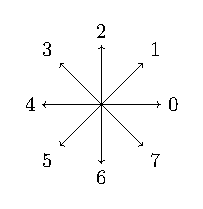
\includegraphics[width=0.3\linewidth]{images/chain-code-dir-num}
    \caption{Example of direction numbers for an 8-directional chain code}
    \label{fig:direction-numbers}
\end{figure}

The code depends on the starting point, but is a circular sequence that can be normalized by letting the starting point be the point that gives the lowest integer value of the sequence. The direction values can also be normalized by using the first difference instead of the absolute direction number.

\subsubsection{Minimum-perimeter polygons (MPPs)}
The goal is to encode the general shape using as few straight segments as possible.

One method is to overlay a coarser grid on the boundary, mark the cells visited by the boundary, and finding the shortest path trough these cells. The hard part is to automate the grid size choice. The algorithm itself is pretty complex stuff.

\subsubsection{Other polygonal approaches}
\paragraph{Merging} This method merges points along a line until the squared sum of errors between the boundary and the line is too large. When the threshold is reached, the procedure repeats with a new line.
\paragraph{Splitting} Start with a line, and find the point that fits the line least. Add that point to the perimeter polygon (now a triangle), and continue until good enough.

\subsubsection{Boundary segments}
It can be useful to separate the boundary into segments. This can be done by finding the convex hull of the shape, and cutting the boundary when it moves in and out of convex deficiencies. See Section \ref{sec:convex-hull}.

For most images, noise etc. will create many small, meaningless convex deficiencies. These can be removed/reduced by smoothing the region, averaging pixels along the boundary, or by using a polygonal approximation.

\subsubsection{Skeletons}
Skeletonizing reduces a shape to a graph, which represents the structural shape of the region. Can be done by thinning (Section \ref{sec:thinning}), but that doesn't ensure connectivity.

The \emph{medial axis transformatian} can be used instead: You have a region $R$ with border $B$. For each point $p \in R$, find its closest neighbor in $B$. If $p$ has more than one such neighbor, it is part of the medial axis. The medial axis then defines the skeleton, which is guaranteed connected. This is computationally heavy to do directly, and there are some more optimized algorithms around.

%%%%%%%%%%%%%%%%%%%%%%%%%%%%%%%%%%%%%%%%%%%%%%%%%%%%%%%%%%%%
\subsection{Boundary descriptors}

\subsubsection{Simple descriptors}
\begin{itemize}
    \item Length: Number of pixels along boundary. For a chain-coded curve: $n\sub{vertical} + n\sub{horizontal} + \sqrt{2} \cdot n\sub{diagonal}$.
    \item Diameter: $\max_{i,j} D(p_i, p_j)$.
\end{itemize}

\subsubsection{Shape numbers}
The shape number of a boundary is the first difference of its chain code, rotated to minimize the integer value. The number of digits of the code defines the order $n$ of the shape number (which is even for a closed boundary).

\subsubsection{Fourier descriptors}
A boundary can be described as a sequence of $K$ points where each point is represented by a complex number:
\begin{equation}
    s(k) = x(k) + \ramuno y(k), \quad k = 0, \dots, K-1
\end{equation}
The DFT and inverse DFT of this is
\begin{equation}
\begin{split}
    a(u) &= \sum_{k=0}^{K-1} s(k) \euler^{- \ramuno 2 \pi \frac{uk}{K}} \\
    s(k) &= \frac{1}{K} \sum_{u=0}^{K-1} a(u) \euler^{\ramuno 2 \pi \frac{uk}{K}}.
\end{split}
\end{equation}
However, if we take the DFT and recreate $s(k)$ with only the first $P$ coefficients, we can get a decent approximation:
\begin{equation}
    \hat{s}(k) = \frac{1}{P} \sum_{u=0}^{P-1} a(u) \euler^{\ramuno 2 \pi \frac{uk}{P}}.
\end{equation}
This is a sort of low-pass filtering. If you simplify to 4 descriptors, you get an ellipse, and with 2 a circle.

\subsubsection{Statistical moments}
Take a boundary segment and rotate it so that the line between its ends is horizontal. The resulting histogram $p(v_i)$ can be described by statistical moments. The mean is
\begin{equation}
    m = \sum_{i=0}^{A-1} v_i p(v_i)
\end{equation}
and the $n$th moment is
\begin{equation}\label{eq:nth-moment}
    \mu_n(v) = \sum_{i=0}^{A-1} (v_i - m)^n p(v_i).
\end{equation}

This essentially describes a boundary as 1D functions.

%%%%%%%%%%%%%%%%%%%%%%%%%%%%%%%%%%%%%%%%%%%%%%%%%%%%%%%%%%%%
\subsection{Regional descriptors}
Regional descriptors are (obviously) used to describe regions rather than boundaries.

\subsubsection{Some simple descriptors}
\begin{itemize}
    \item Area $A$
    \item Perimeter $P$
    \item Compactness $P^2 / A$
    \item Circularity ratio $R_c = 4 \pi A / P^2$
    \item Mean and median intensity
    \item Min and max intensity
    \item Number of pixels over/under mean
\end{itemize}

\subsubsection{Topological descriptors}
Topology is the study of properties unaffected by deformation. Examples are:
\begin{itemize}
    \item The number of holes, $H$.
    \item The number of connected components, $C$.
    \item The \emph{Euler number}, $E = C - H$.
\end{itemize}
We can also extract e.g. the largest connected component of an image.

\subsubsection{Texture}
Textures can be e.g. smooth, coarse, or periodic.

\paragraph{Statistical approaches}
The variance $\sigma^2(z) = \mu_2(z)$ (see \eqref{eq:nth-moment}) is useful, and can be used to define smoothness
\begin{equation}
    R(z) = 1 - \frac{1}{1 + \sigma^2(z)}
\end{equation}
which is $0$ for uniform areas and nearly $1$ for your acne-ridden face.

The 1st (standard deviation), 3rd (histogram skewness), and 4th (relative flatness) moments are also used, and sometimes even higher ones.

Another metric is the \emph{co-occurence matrix} $\M{G} \in \mathbb{Z}^{n \times n}$ for $n$ possible intensity levels. (Group intensities if $\M{G}$ becomes too large.) It is based on a relative position operator, which can be for instance ``one pixel to the right''. Then, if there are, say, 3 occurences of intensity $2$ immediately to the right of intensity $6$, we get $\M{G}_{6,2} = 3$. Then further methods can be used to characterize the co-occurence matrix.

\paragraph{Spectral approaches}
Three Fourier spectrum features are particularly useful:
\begin{itemize}
    \item Prominent peaks give the direction of patterns.
    \item Location of peaks give the spatial period of patterns.
    \item Filtering out periodic features leaves nonperiodic elements which can be analysed statistically
\end{itemize}

To simplify detection and interpretation, you can represent the spectrum in polar coordinates as a function $S(r,\theta)$.

\subsubsection{Moment invariants}
The 2D moment of order $(p+q)$ of an $M \times N$ image is
\begin{equation}
    m_{pq} = \sum_{x=0}^{M-1} \sum_{y=0}^{N-1} x^p y^q f(x,y)
\end{equation}
and the centralized moment is
\begin{equation}
    \mu_{pq} = \sum_{x=0}^{M-1} \sum_{y=0}^{N-1} (x-\bar{x})^p (y-\bar{y})^q f(x,y)
\end{equation}
where
\begin{equation}
    \bar{x} = \frac{m_{10}}{m_{00}}, \quad \bar{y} = \frac{m_{01}}{m_{00}}.
\end{equation}
Then, the \emph{normalized central moments} are
\begin{equation}
    \eta_{pq} = \frac{\mu_{pq}}{\mu_{00}^\gamma} \quad \mbox{with} \quad \gamma = \frac{p+q}{2} + 1
\end{equation}

Based on this, seven moments invariant to translation, scaling, mirroring, and rotation can be formulated. These are the \emph{invariant moments}.

%%%%%%%%%%%%%%%%%%%%%%%%%%%%%%%%%%%%%%%%%%%%%%%%%%%%%%%%%%%%
\subsection[Principal components]{Use of principal components for description}
Principal component analysis is a method of describing data by maximizing variance. The axis that maximizes variance if you project all data points onto it, is the first principal component (PC). That is, the first PC is the axis along which the data is most spread out. All subsequent PCs must be orthogonal to the all other. With many dimensions, you can find $N$ PCs, and describe the data in only those axes. This minimizes the euclidean norm error given the number of axes used.

Each axis is associated with an eigenvalue, and these are nonincreasing from the $n$th to the $(n+1)$th PC. Use this to find which PCs to throw away when you want to reduce dimensionality without damaging the data too much.

\paragraph{Method}
A pixel in an image can be represented as a vector. For an RGB image, this can be $\x = (x_R, x_G, x_B)$. If you gather more data than RGB, the vector will be larger. The mean of all pixel vectors is
\begin{equation}
    \m_{\x} = E\{ \x \} = \frac{1}{K} \sum_{k=1}^K \x_k
\end{equation}
and the covariance is
\begin{equation}
    \M{C}_{\x} = E\left\{ (\x - \m_{\x})(\x - \m_{\x})\T \right\} = \frac{1}{K} \sum_{k=1}^K \x_k \x_k\T - \m_{\x} \m_{\x}\T.
\end{equation}
We can approximate $\x$ by calculating the eigenvectors of $\M{C}_{\x}$, placing them in a matrix $\M{A}$, transforming
\begin{equation}
    \y = \M{A}(\x - \m_{\x}),
\end{equation}
and finally transforming back using a modified $\M{A}$ that only includes the eigenvectors for the $k$ largest eigenvalues:
\begin{equation}
    \hat\x = \M{A}_k\T \y + \m_{\x}
\end{equation}
Then, $\hat\x \in \real{k}$.

%%%%%%%%%%%%%%%%%%%%%%%%%%%%%%%%%%%%%%%%%%%%%%%%%%%%%%%%%%%%
\subsection{Feature parameter fitting using the Hough transform}
The Hough transform can be used to detect and parametrize features such a lines found in an image. It requires an edge image, which can be obtained with e.g. the Canny operator (Section \ref{sssec:adv-edge-detection}). For each edge pixel in the edge image, it loops over parameters for the model, and increments a value for each matching parametrization. The parametrizations with the ``most votes'' will then match features in the image.

A line can be parametrized by two parameters $a$ and $b$
\begin{equation}
    y = mx + b,
\end{equation}
but this gives unbounded $a$, and therefore an unbounded search space of possible parametrizations. Instead, we use the polar parametrization
\begin{equation}
    \rho = x \cos \theta + y \sin \theta,
\end{equation}
where $\rho$ is the shortest distance from the origin to the perpendicular line, and $\theta$ is the angle of the perpendicular, as seen in Figure \ref{fig:polar-line}. Now the parameters are bounded. We can search for any parametrization of a shape, but more parameters require more computation.

\begin{figure}[htbp]
    \centering
    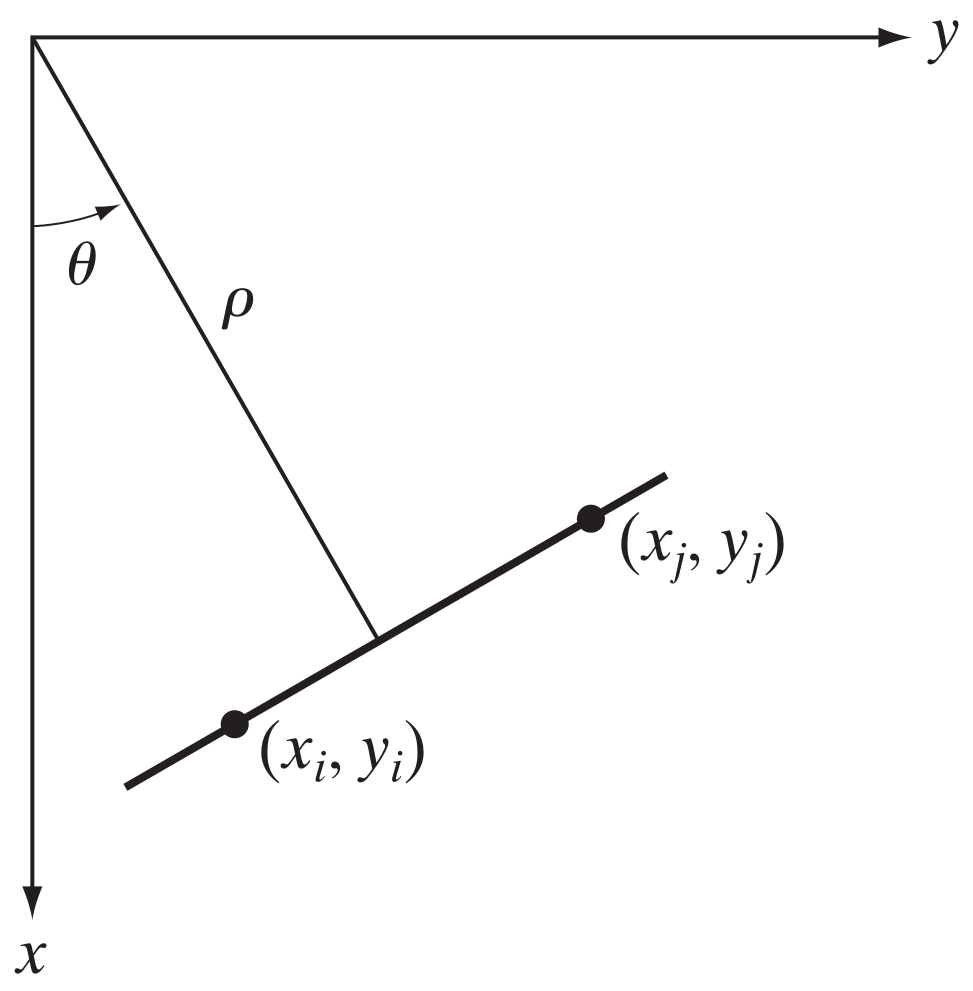
\includegraphics[width=.6\linewidth]{images/R_theta_line}
    \caption{Polar parametrization of a line}
    \label{fig:polar-line}
\end{figure}

%%%%%%%%%%%%%%%%%%%%%%%%%%%%%%%%%%%%%%%%%%%%%%%%%%%%%%%%%%%%
\subsection{Local feature description with SIFT}\label{ssec:sift}
SIFT (scale-invariant feature transform) is an algorithm that detects and describes local features in an image. A rough outline is
\begin{enumerate}
    \item Construct a scale-space: Gaussian-blur the image using increasing $\sigma$ to create a stack of images, ranging from sharp to super blurry. To approximate the LoG, take the difference of each adjacent pair of images. This gives a 3D space in $(x,y,\sigma)$.
    \item Search for local extrema: Max and min values as seen relative to its neighbors in all directions $(x,y,\sigma)$.
    \item Keypoint localization: Use a Taylor series to better find the location of the local extrema. Remove low-contrast keypoints and edge keypoints.
    \item Orientation: Calculate gradient magnitudes in a scale-dependent neighborhood, and put into a gradient histogram. Use this to assign an orientation to the keypoint.
    \item Keypoint descriptor: Use a 16 by 16 neighborhood, divide into 16 blocks, create an 8 bin orientation histogram for each block. You get 128 bin values, which becomes the feature vector of the keypoint.
    \item Matching: Use vector distances to determine matches between descriptors in different images.
\end{enumerate}

%!TEX root = TDT4265-Summary.tex
\section{Object recognition}
Object recognition is the task of finding a specific object within an image.

%%%%%%%%%%%%%%%%%%%%%%%%%%%%%%%%%%%%%%%%%%%%%%%%%%%%%%%%%%%%
\subsection{Patterns and pattern classes}
Patterns are arrangements of descriptors (or ``features''). Pattern recognition is assigning observed patterns to a pattern class. Usually patterns are represented as vectors (quantitative), strings, or trees (structural). When using pattern vectors, the choice of descriptors is super important.

%%%%%%%%%%%%%%%%%%%%%%%%%%%%%%%%%%%%%%%%%%%%%%%%%%%%%%%%%%%%
\subsection[Decision-theoretic methods]{Recognition based on decision-theoretic methods}
Based on decision functions. For pattern classes $\omega_1, \dots, \omega_W$, we need functions $d_1(\x), \dots, d_W(\x)$, so that if $\x$ belongs in class $\omega_i$, then $d_i(\x)$ has the largest value. The decision boundary between two classes are values of $\x$ where two decision functions have the same value.

\subsubsection{Matching}

\paragraph{Minimum distance matching} This method matches candidate vectors $\x$ to prototype vectors $\m$ that represent each class. A candidate belongs to the class with the nearest prototype (``nearness'' measured with some vector norm).

\paragraph{Correlation matching}
Using a template, you can shift it around on an image to find out where it fits best (in the sense of maximum correlation). This can easily be normalized for intensity changes, but not so easily for size and rotation.

\subsubsection{Optimum statistical classifiers}
We can also formulate a classification that is optimal in the sense of minimizing classification errors.

\subsubsection{Neural networks}
Neural networks can be used to classify images and image components. More on this somewhere else.

%%%%%%%%%%%%%%%%%%%%%%%%%%%%%%%%%%%%%%%%%%%%%%%%%%%%%%%%%%%%
\subsection{Feature-based object recognition}
This method depends on a lower-level method to extract features and interest points from images. These can then be matched between images to determine the location of an object. Usually your input is an image of the object alone, and an image of the object in a scene. The output is the location and orientation of the object within the scene. SIFT in Section \ref{ssec:sift} is one way to extract feature descriptors.

\subsubsection{RANSAC}
RANSAC (random sample consensus) is a method of outlier detection that can be used when matching feature vectors between images, to remove false matches. It goes like this:
\begin{enumerate}
    \item Repeat $N$ times:
    \begin{enumerate}
        \item Choose a subset $s \in S$ of points and fit your model to them.
        \item See how many points in $S$ match the model.
    \end{enumerate}
    \item Choose the best fitting model as your result.
\end{enumerate}
Here, $S$ are all your data points. $s$ is a subset large enough to define your model (2 for a line, 8 for a fundamental matrix, etc.). $N$ is a predetermined number of iterations defined to guarantee a certain probability of finding a good model.

RANSAC can do robust estimation (accurate estimation despite many outliers). However, it cannot guarantee with finite $N$ that it finds a good model, it can only guarantee it to a specified probability. It needs very many iterations for sets with many outliers, but variations exist to solve this. The number of iterations necessary to guarantee a good model with probability $p$, given outlier ratio $\epsilon$ is
\begin{equation}
    N = \frac{\log(1-p)}{\log(1-(1-\epsilon)^s)}.
\end{equation}

%!TEX root = TDT4265-Summary.tex
\section{Epipolar geometry}
With one camera, you know the direction to each pixel/object in an image, but not its distance. With two cameras and epipolar geometry, this can be determined.

\begin{figure}[htbp]
    \centering
    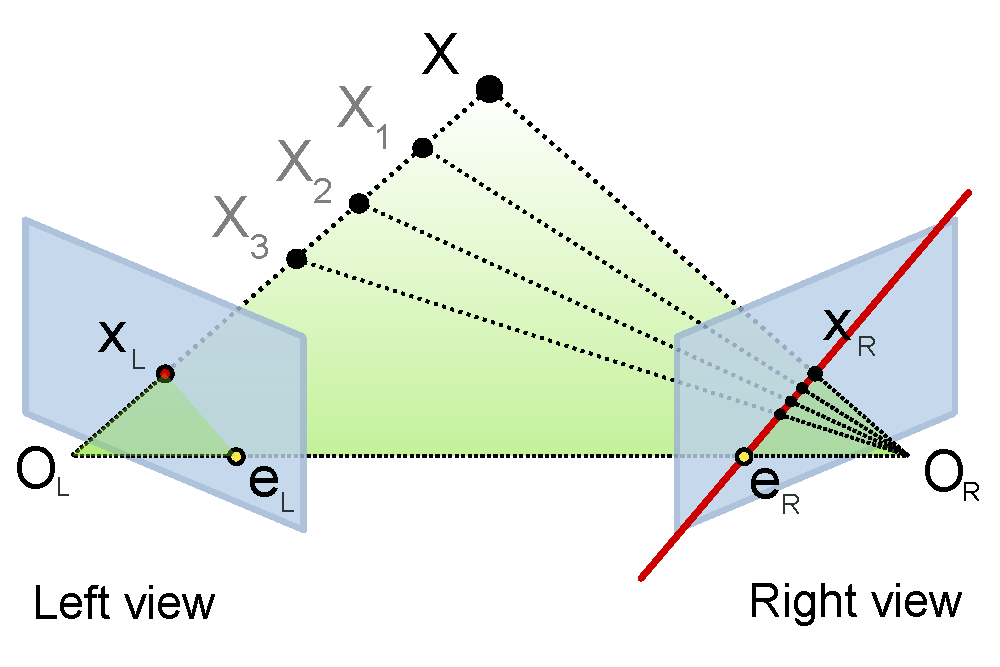
\includegraphics[width=0.95\linewidth]{images/Epipolar_geometry}
    \caption{Epipolar geometry}
    \label{fig:epipolar-geometry}
\end{figure}

In Figure \ref{fig:epipolar-geometry}, both cameras see the object $\V{X}$. The line $\V{O}_L$--$\V{X}$ from the left camera to $\V{X}$, is seen as the epipolar line $\e_R$--$\x_R$ by the right camera, marked in red. (Correspondingly, $\x_L$--$\e_L$ is an epipolar line for the left camera.) This means that $\V{X}$ must lie on the red epipolar line, but we don't know where (this is the fundamental ambiguity). This provides a constraint that can be used to create a model describing the geometric transformation between the two image planes.

\subsection{Essential matrix}
The epipolar constraint from the previous section can be formulated as
\begin{equation}
    \y_1\T \M{E} \y_0 = 0
\end{equation}
where $\y_1$ and $\y_0$ are normalized image coordinates and $\M{E}$ is the essential matrix. This relation holds if the coordinates correspond to the same point in 3D space. Thus, the essential matrix relates points in global coordinates.

\subsection{Fundamental matrix}
The fundamental matrix $\M{F}$ does the same as the essential matrix, but relates points given in image pixel coordinates, such as $\x_L$ and $\x_R$ in Figure \ref{fig:epipolar-geometry}. A similar relation holds for image coordinates that describe the same point in space:
\begin{equation}
    \x_1\T \M{F} \x_0 = 0
\end{equation}

\subsection{Structure from motion (SfM)}
SfM is a method for using data from many 2D images to create a 3D map. It's based on finding features in all the images taken (a huge amount is necessary). Match features between images to estimate camera location, and then pixel distances.

%!TEX root = TDT4265-Summary.tex
\section{Optical flow}
Optical flow is the task of describing how pixels move in an image, thus describing motion of surfaces or objects in an image. Mathematically, you calculate the motion at each pixel position between two frames at times $t$ and $t + \Delta t$.

\subsection{Constraints}
We usually assume constant brightness between frames
\begin{equation}
    I(x,y,t) = I(x + \Delta x, y + \Delta y, t + \Delta t)
\end{equation}
where $I(\cdot)$ is image intensity. We also assume small motion
\begin{multline}
    I(x + \Delta x, y + \Delta y, t + \Delta t) =\\
    I(x,y,z) + \pd{I}{x}\Delta x + \pd{I}{y}\Delta y + \pd{I}{t} \Delta t.
\end{multline}
This gives
\begin{equation}
    \pd{I}{x} V_x + \pd{I}{y} V_y + \pd{I}{t} = 0.
\end{equation}

Determining optical flow can be done in several ways. Sections \ref{ssec:lucas-kanade} and \ref{ssec:horn-schunck} describe differential methods.

\paragraph{Aperture problem} The aperture problem comes from the fact that what a camera sees is only a small part of the world. Motion inside of this frame may appear different than it really is, if the moving object is not contained in the frame.

\subsection{Lucas--Kanade (LK) method}\label{ssec:lucas-kanade}
LK tracks interest points in a scene from one frame to the next. Can use Harris corner points as the interest points. It assumes constant flow in a neighborhood of the pixel examined, and solves the optical flow equations by least squares. Using a neighborhood reduces ambiguities and improves noise performance. But being purely local, it cannot determine flow in the interior of uniform regions.

\subsection{Horn--Schunck (HS) method}\label{ssec:horn-schunck}
A method to estimate optical flow globally. It introduces a global smoothness constraint to solve the aperture problem. It minimizes distortion in flow globally, and prefers solutions that are smoother.

\subsection{Kanade--Lucas-Tomasi (KLT) feature tracker}\label{ssec:kanade-lucas-tomasi}
KLT is a computationally fast feature extraction method that is useful for tracking in realtime video.


\end{document}
